\documentclass{article}
\usepackage[utf8]{inputenc}
\usepackage{float}
\usepackage{amsmath}
\usepackage{amssymb}
\usepackage{physics}
\usepackage{bm}
\usepackage{graphicx}

\newcommand{\bigexp}[2]{\qty(#1)^{#2}}

\author{Kandidatnummer: 15010}
\title{FYS3410 - Module IV}

\begin{document}

\maketitle

\section*{7. }
An electron effective mass in a solid is the apparent mass that an electron has in the solid (i.e. it behaves as if it has that mass when interacting with other particles).
A truncated taylor series for the energy as a function of wavevector can be stated as
$$ \epsilon(k) = \epsilon(K_0) + \dv{\epsilon}{k} (k-k_0) + \tfrac{1}{2}\dv[2]{\epsilon}{k} (k-k_0)^2 + ...$$
We are looking at $k$ in the vicinity of maxima/minima, the first derivative is close to zero and further terms can be neglected as they diminish.
The first term is constant and does not influence the shape or form of the function.
Therefore we can take only the second derivative term into consideration.
We also have an expression given through the dispersion relation

$$ \epsilon(k) = \frac{\hbar^2k^2}{2m} $$

Now combining the two we can solve for the mass

\begin{align*}
	\frac{\hbar^2k^2}{2m} &= \tfrac{1}{2}\dv[2]{\epsilon}{k} (k-k_0)^2\\
	\frac{\hbar^2k^2}{m} &= \dv[2]{\epsilon}{k}k^2\\
	m &= \hbar^2\qty(\dv[2]{\epsilon}{k})^{-1}
\end{align*}

When we consider the electrons as waves we have expressions for the group velocity, $v_g = \pdv{\omega}{k}$, and angular frequency, $\omega = \hbar \epsilon$. We can then do a time dderivation on the expression for group velocity to get the acceleration

\begin{align*}
	a = \dv{v_g}{t} = \frac{1}{\hbar}\dv{}{t}\pdv{\epsilon}{k}\\
	a = \frac{1}{\hbar}\pdv[2]{\epsilon}{k}\pdv{\epsilon}{t}
\end{align*}

In addition we know that $\dv{k}{t} = \frac{F}{\hbar}$ and we can combine this neatly with Newtons second law to get

\begin{align*}
	F=m^*a = \hbar^2\qty(\dv[2]{\epsilon}{k})^{-1}
\end{align*}

\subsection*{a)}
The electron rest mass is a very clean and simple value to measure while the effective mass is a measure of what the electron mass appears to be in a solid. This apparent mass is different from the rest mass because the electron is affected by forces inside for example a crystal and this changes its behaviour when interacting with other particles. In this sense the effective mass is defined through the inertia of the electrons and not graviational mass (the equivalence principle of Einstate states that these should never lead to different masses, however they end up being different in this case as in our model we choose to neglect some forces acting on our electrons and instead adobt them into a change in the effective mass)

\subsection*{b)}
The electrons can have negative effective mass and this is the case for electrons in a band where the band curves downwards away from the maximum. The electrons moves in the opposite direction than it would if it had positive effective mass. It is often beneficial to introduce the concept of "electron holes" as a charge carrier to circumvent this peculiar and slightly awkward effect.

\subsection*{c)}
By using the fact that $E(k) = ak^2$ we can do a derivation and get the answer
\begin{align*}
	m^* &= \hbar^2\bigexp{\dv[2]{\epsilon}{k}}{-1}\\
	m^*&= \hbar^2\bigexp{\dv[2]{}{k}Ak^2}{-1}\\
	m^*&= 2\hbar^2A\\
	m^*&= 1.1\times10^{-32}
\end{align*}

\newpage
\section*{3}

\emph{GaAs is a semiconductor with a direct band gap of ~1.42 eV at room temperature. The
experimental values for the effective masses (in unit of the free electron mass) are: 0.067, 0.082,
and 0.45 for electrons in the conduction band as well as light and heavy holes at the top of the
valence bands, respectively. Compute the corresponding energy dispersion relations and sketch
the band structure of GaAs in the vicinity of $\gamma$ point. What is the origin to have "light" and
"heavy" holes?}

\begin{figure}
	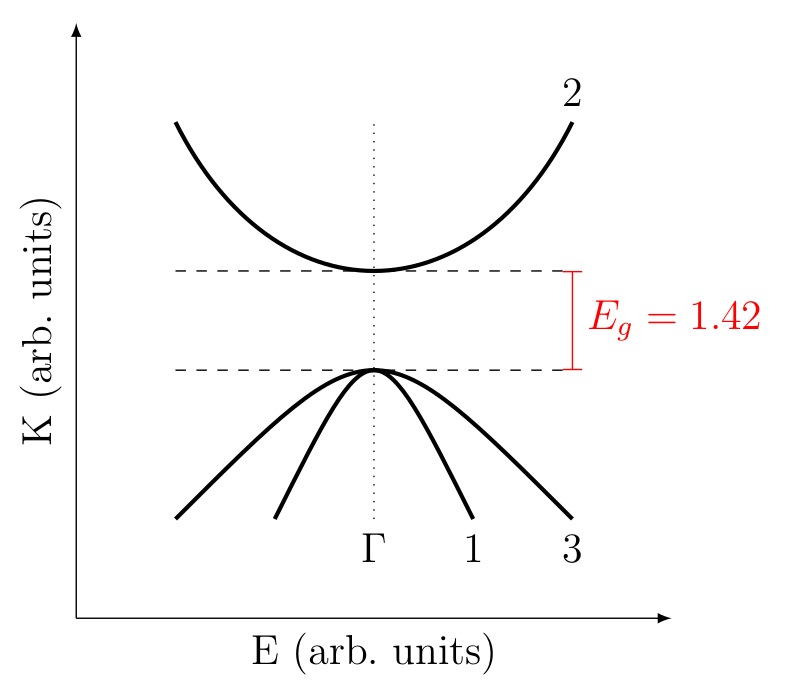
\includegraphics[width = 0.7\linewidth]{bandgap.png}
	\centering
	\caption{Graph of energy dispersion relation for 1.light holes, 2. electrons and 3. heavy holes}
\end{figure}

The energy dispersion relation can be written as
\begin{equation*}
	E'(k) = E(k_0) + \frac{\hbar^2}{2m^*}(k-\gamma)^2
\end{equation*}
From the previous exercise we also have an expression for the effective mass
\begin{equation*}
	\frac{1}{m^*} = \frac{1}{\hbar^2}\pdv[2]{E}{k}
\end{equation*}

Using this, simples calculations gives us the expressions that are plotted.
\begin{align*}
	E_1(k) = E(k_0)-0.09(k-\Gamma)^2\\
	E_2(k) = E(k_0)+0.57(k-\Gamma)^2\\
	E_3(k) = E(k_0)-0.47(k-\Gamma)^2
\end{align*}
An illustration of the different trends can be seen in the figure above.

\end{document}